\documentclass[notitlepage,aps,amsmath,amssymb,11pt]{revtex4-1}
\usepackage{hyperref}
\usepackage{graphicx}

\newcommand{\divv}{\nabla \cdot}
\newcommand{\curl}{\nabla \times}
\newcommand{\curlb}[1]{\left\{ #1 \right\}}
\newcommand{\sqb}[1]{\left[ #1 \right]}
\newcommand{\rndb}[1]{\left( #1 \right)}
\newcommand{\norm}[1]{\left| #1 \right|}
\renewcommand{\vec}[1]{\boldsymbol{#1}}
\newcommand{\tens}[1]{\boldsymbol{#1}}
\newcommand{\diff}[2]{\frac{\rm d#1}{\rm d#2}}
\newcommand{\pdiff}[2]{\frac{\partial#1}{\partial#2}}

\begin{document}

\title{Simulations of Knots in Excitable Media}
\author{Carl Whitfield}
\affiliation{Department of Physics, University of Warwick, Coventry, United Kingdom, CV3 7AL}
\date{\today}
\begin{abstract}
A summary of (and user guide for) simulations of knotted vortex lines in a Fitzhugh-Nagumo reaction-diffusion system in C$++$. I first introduce the problem briefly by discussing relevant background before detailing the contents of the code and outlining some preliminary results.
\end{abstract}
\maketitle
\tableofcontents

\section{Background}

\subsection{Excitable Media and the FitzHugh-Nagumo Model}

An excitable medium is one where the individual constituents can change state due to stimulation by an external cue, such as a chemical concentration. This covers a wide range of systems from biological tissues to wildfires. Of particular interest are excitable media that recover (i.e. can be re-excited), which include many biological examples as well as some chemical reactions. A simple model of the continuum behaviour of such a system is given by the FitzHugh-Nagumo model equations for fields $u$ and $v$
\begin{align}
\label{dudt} \pdiff{u}{t} &= \frac{1}{\epsilon}( u - u^3/3 - v) + \nabla^2 u\\
\label{dvdt} \pdiff{v}{t} &= \epsilon(u + \beta - \gamma v) \, . 
\end{align}
Originally, the model was used to describe axon activity where $u$ is the membrane potential and $v$ a recovery variable \cite{FitzHugh1955, Nagumo1962} and did not include the diffusion term. In the absence of diffusion the equations are a generalised form of the van der Pol oscillator with amplitude of driving $\epsilon$. The inclusion of the diffusion term couples neighbouring oscillators allows travelling wave solutions. Thus this system of equations is commonly used to describe phenomena in various reaction diffusion systems including spiral waves in cardiac tissue. 


\section{Numerical Simulation Code}

\subsection{Outline}

Generating knotted vortex lines in the FitHugh-Nagumo equations requires formulating initial conditions with the correct topology and geometry. This is achieved using a continuous circle-valued function $\Phi$ with a singularity located along the knotted curve $K$ that we wish to initialise, around which $\Phi$ winds by $2 \pi$. The initial conditions for $u$ and $v$ are then given by \cite{Sutcliffe2003}
\begin{align}
\label{uinit} u_0 &= \cos{\Phi} - 0.4\\
\label{vinit} v_0 &= \sin{\Phi} - 0.4 \, .
\end{align}
The offset $-0.4$ is the approximate value of $u$ and $v$ at the centre of the scroll wave core, and approximately the average value about which $u$ and $v$ oscillate. Not only does this mean that locally around the filament, the $u$ and $v$ fields resemble a scroll wave (figure ... ) but also they have matching topology. Wavefronts of $u$ and $v$ form orientable surfaces bounded only by the knot curve (Seifert surfaces). Similarly, the `function' $\Phi$ foliates all of space with a family of Seifert surfaces, therefore the wavefronts of $u_0$ and $v_0$ are also Seifert surfaces.

The phase $\Phi$ is calculated as the scalar potential of a curl-free magnetic field (or equivalently an irrotational flow in a inviscid fluid) around a current carrying wire $K$ with position vector $\vec{l}$ via the Biot-Savart law:
\begin{align}
\label{phik} \Phi = \int_{\vec{r}_0}^{\vec{r}} \vec{B}(\vec{r}') . {\rm d} \vec{r}'
\end{align}
where
\begin{align}
\label{B} \vec{B}(\vec{r}) = \frac{1}{2} \int_K \frac{(\vec{r} - \vec{l})\times {\rm d} \vec{l}}{\norm{\vec{r} - \vec{l}}^3} \, .
\end{align}
Thus, our chosen $\Phi$ is harmonic as well as having the desired topological properties. By Stokes' theorem, the integral can be rewritten in terms of a surface integral
\begin{align}
\label{phis} \Phi = \frac{1}{2} \int_S \frac{( \vec{l} - \vec{r} )}{\norm{ \vec{l} - \vec{r} }^3 }\cdot {\rm d} \vec{S} \, .
\end{align}

On initialisation the simulation code defines the grid of points discretising the three-dimensional domain to be simulated. The size of the box in the $x$ direction is defined by \verb'size' ($L$) and the number of points discretising this direction by \verb'Nx' ($N_x$) such that the spatial step size $h = L/(N_x-1)$. The size of the box in $y$ and $z$ is then just $N_y h$ and $N_z h$ so that the grid spacing is uniform in all directions. Arrays defining quantities on this grid (\emph{e.g.} \verb'phi') are one dimensional, with entries $n = N_z ( N_y i + j) + k$ where $i,j,k$ are the indices for the $x,y,z$ coordinates respectively. Usually, loops over the whole array are of the format
\begin{verbatim}
for(i=0;i<Nx;i++)
{
      for(j=0; j<Ny; j++)
      {
          for(k=0; k<Nz; k++)
          {
               n = pt(i,j,k);
               .....
          }
     }
}
\end{verbatim} 
where the inline function \verb'pt' simply returns the one-dimensional index $n$. Henceforth we will use subscript $n$ or $i,j,k$ to denote array indices on the three-dimensional grid, depending on the context.

\subsection{Initialisation Method I: Surface Integral}

Seifert surfaces have been created by hand using Surface Evolver to triangulate and refine the surface with a fixed boundary curve (generally obtained from KnotPlot). These are stored as \verb'.stl' files, which simply list the properties of each triangular face in the following format
\begin{verbatim}
facet normal nx ny nz
   outer loop
     vertex v1x v1y v1z
     vertex v2x v2y v2z
     vertex v3x v3y v3z
   endloop
  endfacet
\end{verbatim}
where \verb'ni' is the $i$th component of the (normalised) vector normal to the face and \verb'vij' is the $jth$ component of the position vector of the $i$th vertex (all given in floating point format). This is read by the C++ code via the function \verb'init_from_surface_file'. This currently requires only 2 variables as input, the filename of the \verb'.stl' file and a pointer to a vector of the structure \verb'triangle' (both of which are declared as a global variables in the code). The structure \verb'triangle' is defined
\begin{verbatim}
struct triangle
{
    double xvertex[3];  
    double yvertex[3];   
    double zvertex[3];   
    double normal[3];   
    double area;      
    double centre[3];  
};
\end{verbatim}
such that \verb'xvertex' stores the x-components of the 3 vertices, \verb'normal' stores the components of the normal vector, \verb'area' stores the area of the triangle and \verb'centre' the components of the centroid of the triangle. 

The function \verb'init_from_surface_file' reads in the values for the vertices and normals until it reaches the \verb'endsolid' tag at the end of the \verb'.stl' file, storing the total number of faces in $N_K$ (\verb'NK' in the code). Generally the index used to denote the triangle is \verb's' in the code, so we will use subscript $s$ to indicate quantities of the triangle. The centroid is then simply calculated as the mean of the vertices. The function also records the maximum and minimum $x$, $y$ and $z$ coordinates of vertices on the surface as \verb'minxin' ($x^{\rm min}$), \verb'maxxin' ($x^{\rm max}$) \emph{etc.} All surface points $\vec{r}_s$ are then transformed
\begin{align}
\label{rxs} r^{(x)}_s = \frac{X^{\rm max}}{x^{\rm max} - x^{\rm min}}\biggl[r^{(x)}_s - \frac{1}{2}\bigl(x^{\rm max} + x^{\rm min}\bigr)\biggr] \\
\label{rys} r^{(y)}_s = \frac{Y^{\rm max}}{y^{\rm max} - y^{\rm min}}\biggl[r^{(y)}_s - \frac{1}{2}\bigl(y^{\rm max} + y^{\rm min}\bigr)\biggr]  \\
\label{rzs} r^{(z)}_s = \frac{Z^{\rm max}}{z^{\rm max} - z^{\rm min}}\biggl[r^{(z)}_s - \frac{1}{2}\bigl(z^{\rm max} + z^{\rm min}\bigr)\biggr] 
\end{align}
where ($X^{\rm max}$, $Y^{\rm max}$, $Z^{\rm max}$) are the user defined bounds for the knot size (\verb'xmax',\verb'ymax',\verb'zmax'). The surface normal is then scaled accordingly:
\begin{align}
n^{(x)}_s &= n^{(x)}_s\frac{Y^{\rm max} Z^{\rm max}}{\bigl(y^{\rm max} - y^{\rm min}\bigr)\bigl(z^{\rm max} - z^{\rm min}\bigr)}\\
n^{(y)}_s &= n^{(y)}_s\frac{X^{\rm max} Z^{\rm max}}{\bigl(x^{\rm max} - x^{\rm min}\bigr)\bigl(z^{\rm max} - z^{\rm min}\bigr)}\\
n^{(z)}_s &= n^{(z)}_s\frac{X^{\rm max} Y^{\rm max}}{\bigl(x^{\rm max} - x^{\rm min}\bigr)\bigl(y^{\rm max} - y^{\rm min}\bigr)}
\end{align}
and then normalised. Finally, the area of triangle $n$ is calculated from the vertices (Heron's formula):
\begin{align}
A_s &= \sqrt{p(p-r_{21})(p-r_{20})(p-r_{10})} 
\end{align}
where $p = (r_{21} + r_{20} + r_{10})/2$ and $r_{ij} = \norm{\vec{r}_i - \vec{r}_j}$ and $\vec{r}_i$ are the vertices of the triangles. 

The code next calls \verb'initialise_knot' which in turn calls \verb'phi_calc' where the phase field $\Phi$ is calculated at every point in the domain. The surface integral of equation \eqref{phis} is approximated by 
\begin{align}
\label{phin} \Phi_{n} = \sum_{s=0}^{N_K}  \frac{(\vec{c}_s - \vec{x}_{n})}{\norm{\vec{c}_s - \vec{x}_{n}}^3}\cdot \hat{\vec{n}}_s A_s
\end{align}
where $\vec{c}_s$ is the position vector of the centre of triangle $s$. $\Phi_n$ is calculated for all $n$, but contributions to the sum in \eqref{phin} where $\norm{\vec{c}_s - \vec{x}_{n}} = 0$ are skipped. Then, as $\Phi$ is circle valued we redefine it to lie in the range $\Phi \in [-\pi,\pi]$. The resulting $\Phi$ field should be a foliation of the three-dimensional domain with the knot as its boundary, an example plot of level-sets of $\Phi$ is given in figure \ref{fig:phi}.
\begin{figure}[h!]
\centering
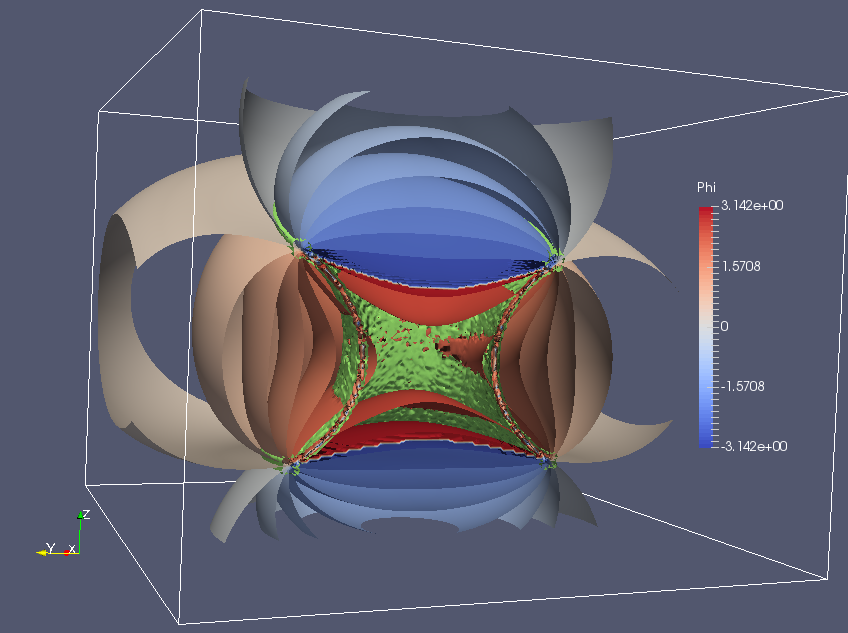
\includegraphics[width=0.8\columnwidth]{phi.png}
\caption{Level-set surfaces of the function $\Phi$ sliced along the $y$ direction for visibility. The green surface shows the input surface (which has an unlink as its boundary). }
\label{fig:phi}
\end{figure}

\subsection{Initialisation Method II: Line Integral}

The option \verb'FROM_KNOT_FILE' indicates that the phase field $\phi$ should be calculated by line integral via the function \verb'init_from_knot_file'. This takes a \verb'.txt' file with a list of point coordinates as input for the knot curve storing them in the vectors \verb'px', \verb'py', \verb'pz' and and also storing the maximum and minimum values of the $x$, $y$ and $z$ components in this list as \verb'minxin', \verb'maxxin' \emph{etc}. The knot curve position vector $(xt,yt,zt)$ is then scaled accordingly as in equations \eqref{rxs}, \eqref{rys} and \eqref{rzs}.

This curve is then further subdivided by linear interpolation between the points to have $N_k =  2 L / h $ (rounded to nearest integer) points, stored in the (vector) arrays \verb'X', \verb'Y' and \verb'Z'. We refer to the position vector of each point as $\vec{l}_s = (X_s, Y_s, Z_s)$. 

The magnetic field is then computed by the function \verb'B_field_calc' called by \verb'initial_cond' at all points on an $N_x \times N_y \times N_z$ grid by summing this quantity over all the points on the loop $s=(1..N_k)$ according to equation \eqref{B}:
\begin{align}
\vec{B}_{i,j,k} = \sum_{s=1}^{N_k} \frac{(\vec{x}_{i,j,k}-\vec{l}_s) \times {\rm d}\vec{l}_s}{\norm{\vec{r}_{i,j,k}-\vec{l}_s}^3}
\end{align}
where $d \vec{l}_s = (d \vec{l}_{s+1} - d \vec{l}_{s-1})/2$. \\

Finally the scalar potential $\Phi$ is computed at all points by the path integral in equation \eqref{phik} for all points. We choose the initial point $\vec{r}_0$ to be the origin of our coordinate system and set $\phi=0$ at $\vec{r}=\vec{r}_0$. To save computation time, we first calculate the path integral on the vertices of the 3-dimensional domain filling in all the values of $\Phi$ on the chosen path in the process, and looping inwards (skipping points that are already filled). {\bf This integral could perhaps be sped up more by looping over the faces of the domain first in this manner and working inwards, as this should assign most points in the domain relatively quickly.} Given a path of $N_p$ gridpoints $(i_p, j_p, k_p)$ connecting $\vec{r}_0$ to the destination point $\vec{r}$, $\Phi$ is computed iteratively along the path as:
\begin{align}
\Phi_{i_p,j_p,k_p} = \Phi_{i_{p-1},j_{p-1},k_{p-1}}  + \frac{1}{2}(\vec{B}_{i_p,j_p,k_p} + \vec{B}_{i_{p-1},j_{p-1},k_{p-1}})\cdot(\vec{r}_{i_p,j_p,k_p} - \vec{r}_{i_{p-1},j_{p-1},k_{p-1}}) 
\end{align}
for $p \in [1:N_p-1]$ where $\Phi_{0,0,0}=0$ and $(i_0,j_0,k_0) = 0$.

The path from the origin to the point in question is found by the function \verb'pathfind'. It was found that simple straight-line paths can give rise to significant numerical errors resulting in incorrect initialisation when the paths come within some small neighbourhood of the knot curve (of approximately one `core diameter' $d_0 = \lambda/\pi$). To avoid these points we fill an empty array \verb'ignore' (or $I$) with the value 1 at every gridpoint where $\norm{\vec{r}_{i,j,k}-\vec{l}_s} < d_0$ for any $s=0..N_k-1$ of the initial curve (this array is computed once during the magnetic field calculation). 

In order to compute the path itself from $\vec{i}_0 = (i_0, j_0, k_0)$ to $\vec{i}_f = (i_f,j_f,k_f)$ we iteratively choose neighbouring gridpoints that are not forbidden. At any point on the path point $\vec{i}_s$ (so long as $(i_s,j_s,k_s) \neq (i_f,j_f,k_f)$, otherwise the pathfinding is complete) we define a preferred direction $\vec{p} = ({\rm sgn}(i_f-i_s),{\rm sgn}(j_f-j_s),{\rm sgn}(k_f-k_s))$, then if the point corresponding to $\vec{i}_s+\vec{p}$ (where $\vec{i}_s=(i_s,j_s,k_s)$) is free to move into, this becomes the next point in the path. Note that a path is forbidden from revisiting a previous point, each time a point is visited the zero array \verb'track' (or $T$) is changed so that  $T_{i_s,j_s,k_s} = 1$. If, this point is blocked ($I_{\vec{i}_s+\vec{p}}=1$ or $T_{\vec{i}_s+\vec{p}}=1$) then instead we sample all neighbouring points and choose the one that maximises a particular weight function $W$. We choose $W$ to be the sum of the alignment with direction to final point and alignment to the magnetic field (which helps to avoid the path spiralling around when it hits an obstacle) as follows,
\begin{align}
W &= \rndb{ \frac{\vec{i}_f-\vec{i}_{s'}}{\norm{\vec{i}_f-\vec{i}_{s'}}} + \frac{\vec{B}_{i_{s'},j_{s'},k_{s'}}}{\norm{\vec{B}_{i_{s'},j_{s'},k_{s'}}}} }\cdot \frac{\vec{i}_{s'}-\vec{i}_{s}}{\norm{\vec{i}_{s'}-\vec{i}_{s}}} \, ,
\end{align}
where $s'$ denotes the neighbouring point in question. If no neighbour points are viable, we step back to the previous point on the path and repeat the previous step, now with the dead-end point unable to be revisited as $T = 1$ at that point. This process is continued until the path is complete or it returns to the origin or the number of points in the path exceeds a large value, in which case the algorithm quits and fails to perform a path integral to this point.

\subsection{Initialisation from file}

There is also the option to initialise a simulation from a previous run of the code. One can initialise from the \verb'phi.vtk' file outputted after calculation of the $\Phi$ field using the option \verb'FROM_PHI_FILE' and defining the string variable \verb'B_filename' as the local path to the input \verb'.vtk' file. This \verb'phi.vtk' file must be from a previous run of the code with the same grid size and spacing settings. 

Similarly, one can continue from the Fitzhugh-Nagumo variables $u$ and $v$ using option \verb'FROM_UV_FILE' and setting \verb'B_filename' as the local path to the input \verb'.vtk' file. Again, this \verb'uv_plotXXX.vtk' file should be from a previous run of the code with the same grid size and spacing settings.  In this case, it may be desirable to start the time counter from the last point of the previous run of the code, in which case set \verb'starttime' $=$ XXX. Otherwise \verb'starttime' should be set to zero. 

\section{FitzHugh-Nagumo Dynamics}

Once $\Phi$ is calculated the Fitzhugh-Nagumo variables are initialised in \verb'uv_initialise' as given by equations \eqref{uinit} and \eqref{vinit}. If initialisation method II is used (\verb'FROM_KNOT_FILE') then $u$ and $v$ are set to -0.4 in the regions that are skipped (as this is the approximate value they take at the centre of the scroll wave:
\begin{verbatim}
for(n=0; n<Nx*Ny*Nz; n++)
{
    u[n] = (2*cos(phi[n]) - 0.4);
    v[n] = (sin(phi[n]) - 0.4);
    if(option==FROM_KNOT_FILE && missed[n]==1)
    {
        u[n] = -0.4;
        v[n] = -0.4;
    }
}
\end{verbatim}

Following initialisation the code iterates the FitzHugh-Nagumo dynamics through time with time spacing \verb'dtime'. There are two method options in the code for this, set by the value of the preprocessor parameter \verb'RK4'. If \verb'RK4' is nonzero then the fourth-order Runge-Kutta method is used (function call \verb'uv_update'), otherwise a simple Euler forward method is employed (function call \verb'uv_update_euler'). In both cases, a simple central difference scheme is used to approximate the Lagrangian of $u$:
\begin{align}
\nabla^2 u_{i,j,k} \approx \frac{1}{h^2} ( u_{i-1,j,k} + u_{i,j-1,k} + u_{i,j,k-1} - 6 u_{i,j,k} + u_{i+1,j,k} +  u_{i,j+1,k}  +  u_{i,j,k+1} ) \, . 
\end{align}
The boundary conditions are usually taken to be of the Neumann type, i.e. $\nabla u = 0$ at the wall. We take the walls to be positioned half a gridspace before the first gridpoint, and half a gridspace after the final gridpoint so that Neumann boundary conditions demand
\begin{align}
u_{-1, j, k} = u_{0,j,k}\\
u_{N_x, j, k} = u_{N_x-1,j,k}
\end{align}
and likewise for the $y$ and $z$ directions. This is incorporated into the code by the function \verb'incw(int i, int p, int N)' which is used to take increments of $i,j,k$ around the current gridpoint. The function returns $i+p$ unless that is outside the range $[0:N-1]$ in which case the counter is `reflected' back into the domain
\begin{verbatim}
inline int incw(int i, int p, int N)   
{
    if(i+p<0) return (-(i+p+1));
    if(i+p>N-1) return (2*N-(i+p+1));
    return (i+p);
}
\end{verbatim} 
Currently, by setting the boolean parameter \verb'periodic' as true then this changes the boundary conditions to periodic {\bf in the z direction only}. Then, the periodic increment function \verb'incp(int i, int p, int N)' is used
\begin{verbatim}
inline int incp(int i, int p, int N)   
{
    if(i+p<0) return (N+i+p);
    else return ((i+p)%N);
}
\end{verbatim} 
in which case the counter continues back at $0$ if it goes above $N-1$ and \emph{vice versa}. To switch to fully periodic boundaries all occurences of \verb'incw' should be replaced by \verb'incp'.

\subsubsection{Euler-forward update}

The Lagrangian of u is stored in the array \verb'D2u' and once this is defined everywhere $u$ and $v$ are updated by the discretised versions of equations \eqref{dudt} and \eqref{dvdt} 
\begin{align}
u^{t+\delta t}_{i,j,k} &= u^{t}_{i,j,k} + \delta t \sqb{ \frac{1}{\epsilon} \rndb{u^{t}_{i,j,k} - \frac{1}{3}(u^{t}_{i,j,k})^3 - v^{t}_{i,j,k}} + \nabla^2 u^{t}_{i,j,k}}\\
v^{t+\delta t}_{i,j,k} &= v^{t}_{i,j,k} + \epsilon \delta t \rndb{ u^{t}_{i,j,k} + \beta - \gamma v^{t}_{i,j,k} } \, .
\end{align}
where the superscript indicates the time at which these quantities are defined.

\subsubsection{Runge-Kutta update}

In this method there is 3 extra `correction' steps after the initial `predictor' update which help to stabilise the dynamics at large values of $\delta t$ (\verb'dtime'). This involves 3 intermediate updates of $u$ and $v$ which we denote with superscripts $t+\delta t/4$,  $t+\delta t/2$ and $t+3\delta t/4$ (although the steps do not correspond to these times) such that
\begin{align}
u^{t+\delta t / 4}_{i,j,k} &= u^{t}_{i , j, k} + \frac{\delta t}{2} f\rndb{u_{i,j,k}^t, v_{i,j,k}^t} \\
u^{t+\delta t / 2}_{i,j,k} &= u^{t}_{i , j, k} + \frac{\delta t}{2} f\rndb{u_{i,j,k}^{t+\delta t / 4}, v_{i,j,k}^{t+\delta t / 4}}\\
u^{t+3\delta t / 4}_{i,j,k} &= u^{t}_{i , j, k} + \delta t \, f\rndb{u_{i,j,k}^{t+\delta t / 2}, v_{i,j,k}^{t+\delta t / 2}}\\
v^{t+\delta t / 4}_{i,j,k} &= v^{t}_{i , j, k} + \frac{\delta t}{2} g\rndb{u_{i,j,k}^t, v_{i,j,k}^t} \\
v^{t+\delta t / 2}_{i,j,k} &= v^{t}_{i , j, k} + \frac{\delta t}{2} g\rndb{u_{i,j,k}^{t+\delta t / 4}, v_{i,j,k}^{t+\delta t / 4}}\\
v^{t+3\delta t / 4}_{i,j,k} &= v^{t}_{i , j, k} + \delta t \, g\rndb{u_{i,j,k}^{t+\delta t / 2}, v_{i,j,k}^{t+\delta t / 2}}
\end{align}
where
\begin{align}
f\rndb{u_{i,j,k}^t, v_{i,j,k}^t} &= \frac{1}{\epsilon} \rndb{u^{t}_{i,j,k} - \frac{1}{3}(u^{t}_{i,j,k})^3 - v^{t}_{i,j,k}} + \nabla^2 u^{t}_{i,j,k} \\
g\rndb{u_{i,j,k}^t, v_{i,j,k}^t} &= u^{t}_{i,j,k} + \beta - \gamma v^{t}_{i,j,k}
\end{align}
These operations are performed in the function \verb'uv_add' where the return value of $f$ and $g$ (at the current intermediate timestep) is stored in the arrays \verb'ku' and \verb'kv' and then the array \verb'kut' and \verb'kvt' keep a running total of their contributions to the final update equations:
\begin{align}
u^{t+\delta t}_{i,j,k} = u^{t}_{i , j, k} + \frac{\delta t}{6} \sqb{ f_{i,j,k}^t + 2 f_{i,j,k}^{t+\delta t / 4}  + 2f_{i,j,k}^{t+\delta t / 2} +  f_{i,j,k}^{t+3\delta t / 4}}\\
v^{t+\delta t}_{i,j,k} = v^{t}_{i , j, k} + \frac{\delta t}{6} \sqb{ g_{i,j,k}^t + 2 g_{i,j,k}^{t+\delta t / 4}  + 2g_{i,j,k}^{t+\delta t / 2} +  g_{i,j,k}^{t+3\delta t / 4}}
\end{align}
where the shorthand $f_{i,j,k}^t = f\rndb{u_{i,j,k}^t, v_{i,j,k}^t}$ is used. Note this method uses approximately twice as much RAM than the Euler forward method due the extra arrays that are necessary.

\subsubsection{Output}

The code tracks the time dependent behaviour of $u$ and $v$ by outputting these fields after every \verb'skiptime' units of time. The \verb'startime'


\subsection{Numerical ``Hummingbird''}

To track the properties of the knotted vortex line we write a function which locates and traces the curve with a one-dimensional array of points, we nickname  this function the ``Hummingbird'' due to Winfree's comment in \cite{Winfree1990}. 

\section{Convergence and Accuracy Tests}

\section{Results}

\section{Future Directions and Open Questions}

\begin{thebibliography}{10}
\bibitem{Maucher2016} F. Maucher and P. Sutcliffe \href{http://dx.doi.org/10.1103/PhysRevLett.116.178101}{Phys. Rev. Lett. {\bf 116}(178101) (2016)}

\end{thebibliography}

\end{document}